\chapter{Introduction to {R}}
\label{chap:RI}

\section{Outline of the the R module} 

You will use R a lot during the rest of your courses, your thesis 
dissertation, and very likely, your career. The {\tt R} module aims to lay 
down the foundations for you to become comfortable with it, specifically,

\begin{compactitem}\itemsep4pt
		\item Giving you an introduction to R syntax and programming 
		conventions, assuming you have never set your eyes on R

    \item Teaching you principles of data processing and exploration 
    (including visualization) using R

    \item Teaching you principles of clean and efficient programming using R

		\item Teaching you how to generate publication quality graphics in R 

		\item Teaching you how to develop reproducible data analysis "work 
	flows" so you (or anybody else) can run and re-run your analyses,
	graphics outputs and all, in R 
\end{compactitem} 


\section{What is {\tt R}?} 

{\tt R} is a freely available statistical software with strong 
programming capabilities widely used by professional scientists around 
the world. It was based on the commercial statistical software {\tt S} 
by Robert Gentleman and Ross Ihaka. The first stable version appeared 
in 2000. 

{\tt R} was essentially designed for {\it programming} statistical 
analysis and data-mining. It became the standard tool for data 
analysis and visualization in biology in a matter of just 10 years or 
so. It is also increasingly being used for modelling in biology. This 
is because 
\begin{enumerate}
\item {\tt R} has many tried and tested packages to perform practically all statistical analysis
\item {\tt R} has numerous packages for data-handling and processing   
\item {\tt R} has excellent graphing and visualization capabilities
\item {\tt R} has good capabilities for mathematical calculations, including matrix algebra 
\end{enumerate}

\section{Why {\tt R}?} 
There are many commercial statistical (minitab, SPSS, etc) software 
packages in the world that are mouse-driven, warm, and friendly, and 
have lots of statistical tests and plotting/graphing capabilities. Why 
not just use them? Here are some very good reasons:
\begin{compactitem}\itemsep4pt
	\item {\tt R} is scriptable, so you can build a perfectly repeatable 
	record of your analysis. This in itself has several advantages:
		\begin{compactitem}\itemsep0pt
			\item You can never replicate {\it exactly} the same analysis with 
			all the same steps using a point-and-click approach/software. 
			With {\tt R} you can reproduce your full analysis for 
			 yourself (in the future!), your colleagues, your 
			 supervisor/employer, and any journal you might want to submit your work to.
			\item You may need to rerun your analysis every time you get new data. 
			Once you have it all in a {\tt R} script, you can just rerun your 
			analysis and go home!
			\item You may need to tweak your analysis many times (new data, 
			supervisor changes mind, you change mind, paper reviewers want 
			you do something differently). Having the analysis recorded as 
			script then allows you to do so by revising the relevant parts of your 
			analysis with relatively little pain.  
		\end{compactitem}
			
	\item {\tt R} provides basically every statistical test you'll ever need 
	and is constantly being improved --  you can tailor your analyses 
	rather than trying to use the more limited options each 
	statistical software package can offer 
	 
	\item {\tt R} can produce publication-quality graphics that can be 
	re-produced with scripts -- you won't get RSI mouse-clicking your 
	way though graphing and re-graphing your data every time you change 
	your analysis!
	  
	\item {\tt R} is freely available for all common computer operating systems 
	-- if you want a copy on your laptop, help yourself 
	at the \href{https://cran.r-project.org}{CRAN} website.

\end{compactitem}

{\it Thus, being able to program in R means you can develop and 
automate your own data handling, statistical analysis, and 
graphing/plotting, a set of skills you are likely to need in many, if 
not most careers paths!}

\subsection{Would you ever need anything other than {R}?} 

Being able to program R means you can develop and automate your 
statistical analyses and the generation of figures into a reproducible 
work flow. For many of you, using R as your only programming 
language will do the job. However, if your work also includes 
extensive numerical simulations, manipulation of very large matrices, 
bioinformatics, relational database access and manipulation, or web 
development, you will be better-off {\it also} knowing another 
programming language that is more versatile and computationally 
efficient (like {\tt python}, {\tt perl} or {\tt C}).

\section{Installing {\tt R}}

If you are using a college computer, {\tt R} will likely already be 
available. Otherwise you can install {\tt R} on your own computer as 
follows:  

On linux/ubuntu, run the following in terminal:
\begin{lstlisting}
sudo apt-get install r-base r-base-dev
\end{lstlisting}

On Mac OS X, download and install from:
\url{https://cran.r-project.org/bin/macosx/}

On Windows, download and install from:
\url{https://cran.r-project.org/bin/windows/base/}

\section{Getting started}

Let's briefly look at the bare-bones {\tt R} interface and command line 
interface (CLI), and then switch to a more Interactive Development 
Environment (IDE) like Geany or RStudio. 

Launch R (From Applications menu on Window or Mac, from terminal in 
Linux/Ubuntu) --- it should look something like this (on Linux/Ubuntu 
or Mac terminal):

\begin{center}
	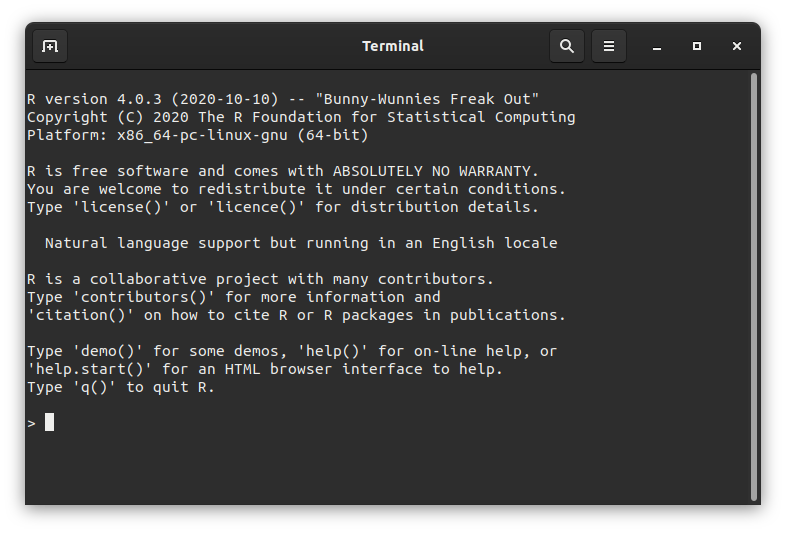
\includegraphics[width=.8\textwidth]{R_Linux.png}
\end{center}

Or like this (Windows "console", similar in Mac):
 
\begin{center}
	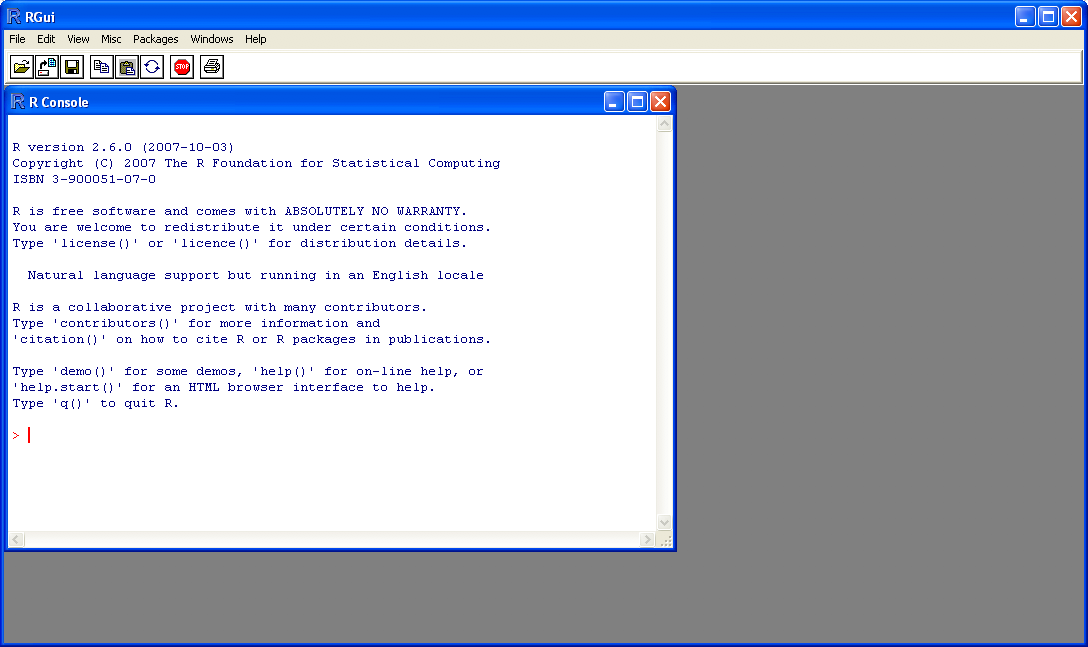
\includegraphics[width=.8\textwidth]{HorrorVacui.png}
\end{center}

\subsection{Gooey IDEs!}

To develop your R code, you should ideally use an IDE (Interactive 
Development Environment) that offers useful features like syntax  
highlighting (google it!) and embedded data and plot viewing windows, 
such as RStudio, {\tt geany}, {\tt vim}, etc. 

These IDEs come with graphic user interfaces (GUI's, or ``gooeys'') of 
differing levels of sophistication and shiny-ness.

In fact, one of the reasons that R has become so popular is that there 
are some very nice, freely available GUI IDE's for it where you can 
use your mouse to do certain ``stuff''. 

In particular, \href{http://rstudio.org/}{RStudio} is very good. 

A big advantage of something like RStudio is that you will get ``syntax 
highlighting'' wherein R language elements such as variables, commands, 
and brackets are differently colored. This is very handy and will make 
your R programming far more convenient and error-free. If you are using 
your own desktop/laptop, you can download it freely from 
\url{https://www.rstudio.com/} and install (versions are available for all 
computer platforms). If you are suing a college computer, it should 
already be available.

The R modules do not require you to use RStudio (everything will 
be command line based), but I would recommend that you to use it, or 
some other IDE like {\tt geany} or {\tt emacs}. 

You may now launch RStudio (assuming it is available on your computer). 
Here is an example RStudio window: 
\begin{center}
	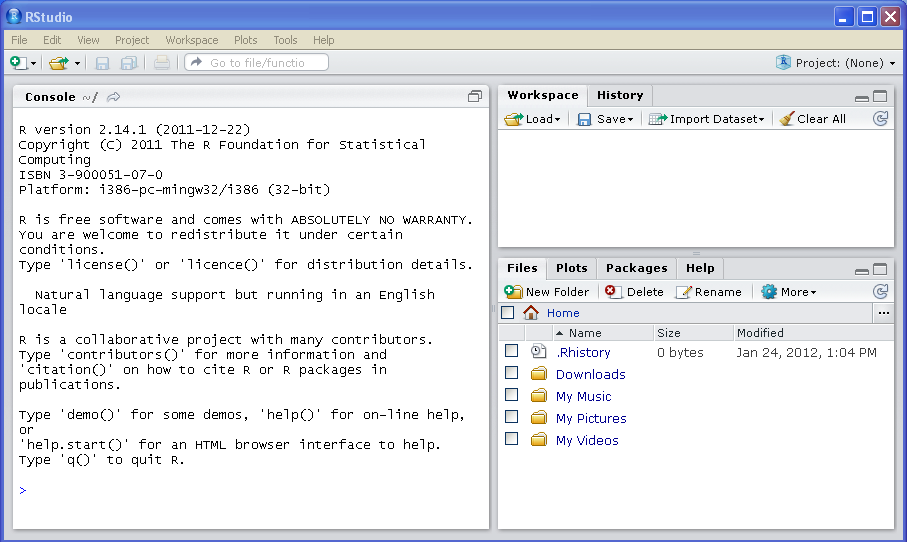
\includegraphics[width=0.8\textwidth]{RStudio.png}
\end{center}

You are still in the R environment, but with some useful frills and 
additional thrills. There are four main elements here (you can hide or 
resize any of them using the RStudio GUI options):

\begin{description}

\item [Console] This is the same R terminal you saw above. In this week 
we will work mainly in this console

\item [Source code] This panel is the code editor with syntax 
highlighting and other handy features that we will explore soon. This 
is where you will write your scripts/programs, and save them. To save, 
you will use {\tt Ctrl + S} and to execute it you will use {\tt Ctrl + Shift + 
S}

\item [Environment] This panel lists all the variables you created 
(more on this later). It has another tab that shows you the history of 
the commands you typed

\item [Plots] This panel shows you all the plots you drew. Other tabs 
in this panel allow you to access the list of packages
you have loaded, and the help page for commands (just type {\tt 
help(command\_name)} in the Console) and packages
\end{description}

In RStudio, you can feed your mouse habit, but I strongly suggest using 
the terminal/console, and resist, to the extent possible, the 
temptation to do everything using the shiny buttons you see (that is 
the dark side pulling, my young {\it padawan}).

\section{Some {\tt R} Basics}

Gets get started with some {\tt R} basics. You will be working by 
entering R commands interactively at the R user prompt ({\tt >}). Up 
and down arrow keys scroll through your command history. 

\subsection{Useful R commands}
\begin{tabular}{p{3cm} p{10cm}} 
	{\tt ls()} & list all the variables in the work space \\
	{\tt rm('a', 'b')} & remove variable(s) {\tt a} and {\tt b}\\
	{\tt rm(list=ls())} & remove all variable(s)\\
	{\tt getwd()} & get current working directory \\
	{\tt setwd('Path')} & set working directory to {\tt Path} \\
	{\tt q()} & quit R \\
	{\tt ?Command} & show the documentation of {\tt Command} \\
	{\tt ??Keyword} & search the all packages/functions with 
	{\tt Keyword}, ``fuzzy search''\\
\end{tabular}\\

\subsection{R Warm-up}

Like in any programming language, you will need to use ``variables'' to 
store information in a R session's workspace. Each Variable has a 
reserved location in your memory (RAM), and takes up ``real estate'' in 
it --- that is when you create a variable you reserve some space in yur 
computer's memory.

Now, try assigning a few variables in the R and doing things to them:
\begin{lstlisting}
> a <- 4  # store 4 as variable a
> a
[1] 4
> a*a  # product
[1] 16
> a_squared <- a*a 
> sqrt(a_squared) # square root
[1] 4
> v <- c(0, 1, 2, 3, 4) # build a vector with c (for "concatenate") 
\end{lstlisting}

Note that any text after a "\#" is ignored by R --- handy for 
commenting. {\it In general, please comment your code and scripts, for 
{\it everybody's} sake}. You will be amazed by how difficult it is to 
read and understand what a certain R script does (or any other script, 
for that matter) without judicious comments --- even scripts you  
yourself wrote not so long ago!

\begin{tipbox}
{\tt c()} (concatenate) is one of the most commonly used 
functions --- it will appear again and again! (try {\tt ?c}). 
\end{tipbox}

OK continuing our R warmup:
\begin{lstlisting}
> v # Display the vector variable you created
[1] 0 1 2 3 4
> is.vector(v) # check if it's a vector
[1] TRUE
> mean(v) # mean
[1] 2
\end{lstlisting}

\begin{tipbox}
Thus, a ``vector'' is like a single column or row in a ``spreadsheet''. Multiple vectors can be combined to make a matrix (the full spreadsheet).  
\end{tipbox}

This is one of many ways R stores and processes data. More on R data 
types and objects below.  

A single value (any kind) is a vector object of length 1 by default. 
That's why in the console you see {\tt [1]} before any single-value 
output (e.g., type {\tt 8}, and you will see {\tt [1] 8}).

\begin{lstlisting}
> var(v) # variance
[1] 2.5
> median(v) # median
[1] 2
> sum(v) # sum all elements
[1] 10
> prod(v + 1) # multiply
[1] 120
> length(v) # length of vector
[1] 5
\end{lstlisting}

\subsection{Variable names and Tabbing}

In R, you can name variables in the following way to keep track of 
related variables:
\begin{lstlisting}
> wing.width.cm <- 1.2 #Using dot notation 
> wing.length.cm <- c(4.7, 5.2, 4.8)
\end{lstlisting}

This can be handy; type:
\begin{lstlisting}
> wing.
\end{lstlisting}

And then hit the {\tt tab} key to reveal all variables in that 
category. This is nice --- variable names should be as obvious as 
possible. However, they should not be over-long either! Good style and 
readability is more important than just convenient variable names. 

\subsection{Operators}
The usual ``operators'' are available in R:

\begin{tabular}{p{2cm} p{11cm}} 
 {\tt +} & Addition \\
 {\tt -} & Subtraction\\
 {\tt *} & Multiplication\\
 {\tt /} & Division\\
 {\tt \textasciicircum} & Power\\
 {\tt \%\%} & Modulo\\
 {\tt \%/\%} & Integer division\\
 {\tt ==} & Equals\\
 {\tt !=} & Differs\\
 {\tt $>$} & Greater\\
 {\tt $>$=} & Greater or equal\\
 {\tt \&} & Logical and\\
 {\tt $\vert$} & Logical or\\
 {\tt !} & Logical not\\
\end{tabular}

\subsection{When things go wrong}

Syntax errors are those where you've just made a mistake while typing 
code. Here are some common problems in {\tt R}: 

\begin{itemize}
\item missing close bracket leads to  continuation line.
\begin{lstlisting}
> x <- (1 + (2 * 3)
+ 
\end{lstlisting}
Hit {\tt Ctrl-C} (UNIX terminal or base R command line) or ESC (in in RStudio) or keep typing!

\item Too many parentheses: {\tt 2 + (2*3))}

\item Wrong or mismatched brackets (see next subsection)

\item Do not mix double quotes and single quotes

\end{itemize}

\begin{tipbox}
	When things are taking too long and the R consile seems frozen, try 
	{\tt Ctrl + C} (UNIX terminal or base R command line) or ESC (in in RStudio) to force an exit from whatever is going on.
\end{tipbox}

\subsection{Types of parentheses}
R has specific uses for different types of parentheses that you need to 
get used to:

\begin{tabular}{p{5cm} p{9.5cm}} 
 {\tt f(3,4)} & call the function (or command) f, with the 
	arguments 3 \& 4. \\
 {\tt a + (b*c)} & to enforce order over which statements 
  or calculations are executed. Here {\tt (b*c)} is executed before 
  adding to {\tt a}; here is an alternative order: {\tt (a + b)*c}\\
 {\tt \{ expr1; expr2; \ldots exprn \}} & group a set of expressions or 
 commands into one compound expression. Value returned is value of last
    expression; used in building function, loops, and conditionals (more on 
    these soon!).\\
 {\tt x[4] } & get the 4th element of the vector {\tt x}.\\
 {\tt li[[3]]} & get the 3rd element of some list {\tt li}, and return it.
    (compare with li[3], which returns a list with just the 3rd element
    inside). More on lists in next section
\end{tabular}

\section{Variable Types}

There are different kinds of data variable types in R, but you will 
basically need to know four for most of your work: integer, float (or 
``numeric'', including real numbers), string (or ``character'', e.g., 
text), and Boolean (``logical''; {\tt True} or {\tt False}).  Try this:

\begin{lstlisting}
> v <- TRUE
> class(v)
[1] "logical"

> v <- 3.2
> class(v)
[1] "numeric"

> v <- 2L
> class(v)
[1] "integer"

> v <- "A string"
> class(v)
[1] "character"
\end{lstlisting}

\begin{tipbox}
R will use {\tt E} notation in outputs of statistical tests to display 
very large or small numbers. If you are not used to different 
representations of long numbers, the {\tt E} notation might be 
confusing. Try this:
\begin{lstlisting}
> 1E4
[1] 10000
> 1e4
[1] 10000
> 5e-2
[1] 0.05
> 1E4^2
[1] 1e+08
> 1 / 3 / 1e8
[1] 3.333333e-09
\end{lstlisting}
Keep and eye out for {\tt E} notation! 
\end{tipbox}

\subsection{Type Conversion and Special Values}
In the following examples, the {\tt as.*} commands all convert a 
variable from one type to another:	
\begin{lstlisting}
> as.integer(3.1)
[1] 3
> as.numeric(4)
[1] 4
> as.roman(155)
[1] CLV
> as.character(155) # same as converting to string
[1] "155"
> as.logical(5) #what's happening here?!
[1] TRUE
> as.logical(0)
[1] FALSE
> b <- NA
> is.na(b)
[1] TRUE
> b <- 0/0
> b
[1] NaN
> is.nan(b)
[1] TRUE
> b <- 5/0
> b
[1] Inf
> is.nan(b)
[1] FALSE
> is.infinite(b)
[1] TRUE
> is.finite(b)
[1] FALSE
> is.finite(0/0)
[1] FALSE
\end{lstlisting}

\begin{tipbox}	
Beware of the difference between {\tt NA} ({\tt N}ot {\tt A}vailable) 
and {\tt NaN} ({\tt N}ot {\tt a} {\tt N}umber)!

R will use {\tt NA} to represent/identify missing values in data or 
outputs, while  {\tt NaN} represent nonsense values (e.g., 0/0) that 
cannot be represented as a number or some other data type. See what R 
has to say about this: try {\tt ?is.nan}, {\tt ?is.na}, {\tt ?NA}, {\tt 
?NaN} in the R commandline (one at a time!).

There are also {\tt Inf} (Infinity, e.g., 1/0), and {\tt NULL} 
(variable not set) value types. Look these up as well using {\tt ?}.
\end{tipbox}

\section{Data Structure types}
R comes with different built-in structures (objects) for data storage and 
manipulation. Mastering these, and knowing which one to use when will 
help you write better, more efficient programs and also handle diverse 
datasets (numbers, counts, names, dates, etc). 

\subsection{Vectors}
The Vector, which you first saw above, is a fundamental data object in 
R. Scalars (single data values) are treated as vector of length 1. {\it 
A vector is like a single column or row in a spreadsheet.} Now get back 
into R (if you somehow quit R using {\tt q()} or something else), and 
try this:
\begin{lstlisting}
> a <- 5
> is.vector(a)
[1] TRUE
> v1 <- c(0.02, 0.5, 1)
> v2 <- c("a", "bc", "def", "ghij")
> v3 <- c(TRUE, TRUE, FALSE)
\end{lstlisting}
{\tt R} vectors can only store data of a single type (e.g., all numeric 
or all character). If you try to combine different types, R will 
homogenize everything to the same data type. To see this, try the 
following:
\begin{lstlisting}
> v1 <- c(0.02, TRUE, 1)
> v1 # TRUE gets converted to 1.00!
[1] 0.02 1.00 1.00
> v1 <- c(0.02, "Mary", 1)
> v1 # Everything gets converted to text!
[1] "0.02" "Mary" "1"
\end{lstlisting}

\subsection{Matrices and arrays} 

A {\tt R} {\tt matrix} is a 2 dimensional vector (has both rows and columns). 
and an {\tt R array} is can store data in more than two dimensions 
(e.g., a stack of 2-D matrices). 

{\tt R} has many functions to build and manipulate matrices and arrays. 
Try:

\begin{lstlisting}	
> mat1 <- matrix(1:25, 5, 5)
> mat1
	 [,1] [,2] [,3] [,4] [,5]
[1,]    1    6   11   16   21
[2,]    2    7   12   17   22
[3,]    3    8   13   18   23
[4,]    4    9   14   19   24
[5,]    5   10   15   20   25
> mat1 <- matrix(1:25, 5, 5, byrow=TRUE)
> mat1
	 [,1] [,2] [,3] [,4] [,5]
[1,]    1    2    3    4    5
[2,]    6    7    8    9   10
[3,]   11   12   13   14   15
[4,]   16   17   18   19   20
[5,]   21   22   23   24   25
> dim(mat1) #get the size of the matrix
[1] 5 5
\end{lstlisting}

Make an array consisting of two 5$\times$5 matrices containing the 
integers 1--50:
\begin{lstlisting}
> arr1 <- array(1:50, c(5, 5, 2))
> arr1
, , 1

	 [,1] [,2] [,3] [,4] [,5]
[1,]    1    6   11   16   21
[2,]    2    7   12   17   22
[3,]    3    8   13   18   23
[4,]    4    9   14   19   24
[5,]    5   10   15   20   25

, , 2

	 [,1] [,2] [,3] [,4] [,5]
[1,]   26   31   36   41   46
[2,]   27   32   37   42   47
[3,]   28   33   38   43   48
[4,]   29   34   39   44   49
[5,]   30   35   40   45   50
\end{lstlisting}

Just like {\tt R} vectors, {\tt R} matrices and arrays have to be of a 
homogeneous type, and R will do the same sort of type homogenization 
you saw for R vectors above (try inserting a text value in {\tt mat1} and 
see what happens), and in {\tt python}'s {\tt numpy} array and matrix 
data structures. 

\subsection{Data frames}

This is a very important data structure in {\tt R}. Unlike matrices and 
vectors, {\tt R} data frames can store data in which each column 
contains a different data type (e.g., numbers, strings, boolean) or 
even a combination of data types, just like a standard spreadsheet. 
Indeed, the dataframe data type was built to emulate some of the 
convenient properties of spreadsheets. Many statistical and plotting 
functions and packages in R naturally use data frames. Let's build and 
manipulate a dataframe:
\begin{lstlisting}
> Col1 <- 1:10
> Col1
 [1]  1  2  3  4  5  6  7  8  9 10
> Col2 <- LETTERS[1:10]
> Col2
 [1] "A" "B" "C" "D" "E" "F" "G" "H" "I" "J"
> Col3 <- runif(10) # 10 random numbers from a uniform distribution
> Col3
 [1] 0.29109 0.91495 0.64962 0.95503 0.26589 0.02482 0.59718
 [8] 0.99134 0.98786 0.86168
> MyDF <- data.frame(Col1, Col2, Col3)
> MyDF
	 Col1 Col2      Col3
1     1    A 0.2910981
2     2    B 0.9149558
3     3    C 0.6496248
4     4    D 0.9550331
5     5    E 0.2658936
6     6    F 0.0248217
7     7    G 0.5971868
8     8    H 0.9913407
9     9    I 0.9878679
10   10    J 0.8616854
> names(MyDF) <- c("A.name", "another", "another.one")
> MyDF
	 A.name another another.one
1       1       A   0.2910981
2       2       B   0.9149558
3       3       C   0.6496248
4       4       D   0.9550331
5       5       E   0.2658936
6       6       F   0.0248217
7       7       G   0.5971868
8       8       H   0.9913407
9       9       I   0.9878679
10     10       J   0.8616854
\end{lstlisting}

Unlike matrices, you can access the contents of data frames by naming 
the columns using a \$ sign: 
\begin{lstlisting}
> MyDF$A.name
 [1]  1  2  3  4  5  6  7  8  9 10
> MyDF[,1] #using numerical indexing instead
 [1]  1  2  3  4  5  6  7  8  9 10
> MyDF[c("A.name","another")] # show two specific columns only
	 A.name another
1       1       A
2       2       B
3       3       C
4       4       D
5       5       E
6       6       F
7       7       G
8       8       H
9       9       I
10     10       J
\end{lstlisting}

You can check whether a particular object is a dataframe data structure with:
\begin{lstlisting}
> class(MyDF)
[1] "data.frame"
\end{lstlisting}
You can check the structure of a dataframe with {\tt str()}:
\begin{lstlisting}
> str(MyDF)
'data.frame':	10 obs. of  3 variables:
 $ A.name     : int  1 2 3 4 5 6 7 8 9 10
 $ another    : Factor w/ 10 levels "A","B","C","D",..
 $ another.one: num  0.291 0.915 0.65 0.955 0.266 ...
\end{lstlisting}
You can print the column names and top few rows with {\tt head()},
\begin{lstlisting}
> head(MyDF)
\end{lstlisting}

And the bottom few rows with {\tt tail()},
\begin{lstlisting}
> tail(MyDF)
\end{lstlisting}

\begin{tipbox}
	What is the ``factor'' data type in the data frame you created? You 
	will see that R may mysteriously convert certain columns in dataframes 
	to a factor type, which has "levels".  
	
	R has a special data type called `factor'. It basically considers 
	columns containing strings-only in a data frame to be a grouping 
	variable. You can convert vectors to and from the {\tt factor} class. 
	Try the following:
	
	\begin{lstlisting}
	> a <- as.factor(2)
	> a
	[1] 2
	Levels: 2
	> class(a)
	[1] "factor"
	\end{lstlisting}	
\end{tipbox}

\subsection{Lists} 

A list is used to collect a group of data objects of different sizes 
and types (e.g., one whole data frame and one vector can both be in a 
single list). It is simply an ordered collection of objects (that can 
be variables). The outputs of many statistical functions in R are lists 
(e.g. linear model fitting using {\tt lm()}), to return all relevant 
information in one output object. So you need to know how to unpack and 
manipulate lists. 

\begin{tipbox}	
As a budding multilingual quantitative biologist, you should not be 
perturbed by the fact that a {\tt list} is a very different data structure in 
python vs R!
\end{tipbox}
	
\begin{lstlisting}
> List1 <- list(species=c("Quercus robur","Fraxinus excelsior"), age=c(123, 84))
> List1
$species
[1] "Quercus robur"      "Fraxinus excelsior"

$age
[1] 123 84
\end{lstlisting}

You can access contents of a list item using number of the item instead of name:
\begin{lstlisting}
> List1[[1]]  
[1] "Quercus robur"      "Fraxinus excelsior"
> List1[[2]]
[1] 123 84
\end{lstlisting}

And you can access it using the name of the item in these two way:
\begin{lstlisting}
> List1[["age"]]
[1] 123 84
> List1$age
[1] 123 84
\end{lstlisting}

You can build lists of lists too! Also, you have perhaps guessed by now 
that {\tt R} dataframes are actually a kind of list.

\begin{tipbox}
If dataframes are so nice, why use {\tt R} matrices at all? The problem 
is that dataframes can be too slow when large numbers of mathematical 
calculations or operations need to be performed. In such cases, you 
will need to convert a dataframe to a matrix. But for statistical 
analyses and plotting, data frames will get the job done.          
\end{tipbox}

\section{Creating and manipulating data structures}
 
\subsection{Creating Sequences}

The {\tt :} operator creates vectors of sequential integers:

\begin{lstlisting}
> years <- 1990:2009
> years
[1] 1990 1991 1992 1993 1994 1995 1996 1997 1998 1999
[11] 2000 2001 2002 2003 2004 2005 2006 2007 2008 2009

> years <- 2009:1990 # or in reverse order 
> years
[1] 2009 2008 2007 2006 2005 2004 2003 2002 2001 2000
[11] 1999 1998 1997 1996 1995 1994 1993 1992 1991 1990
\end{lstlisting}

For sequences of fractional numbers, you have to use {\tt seq()} :

\begin{lstlisting}
> seq(1, 10, 0.5)
 [1]  1.0  1.5  2.0  2.5  3.0  3.5  4.0  4.5  5.0  5.5  6.0  6.5  7.0  7.5  8.0
[16]  8.5  9.0  9.5 10.0
\end{lstlisting}

You can also {\tt seq(from=1,to=10, by=0.5)} OR {\tt seq(from=1, 
by=0.5, to=10)} with the same effect (try it) --- this explicit, 
"argument matching" approach is partly why {\tt R} is so popular.

\subsection{Acessing parts of data stuctures -- Indices and Indexing}
Every element (entry) of a vector in R has an order: the first value, 
second, third, etc. To illustrate this, let's create a simple vector:
\begin{lstlisting}
> MyVar <- c( 'a' , 'b' , 'c' , 'd' , 'e' )
\end{lstlisting}
Then, square brackets extract values based on their numerical order 
in the vector:
\begin{lstlisting}
> MyVar[1] # Show element in first position 
[1] "a"
> MyVar[4]
[1] "d" # Show element in fourth position 
\end{lstlisting}
The values in square brackets are called "indices" --- they 
give the index (position) of the required value. We can also select 
sets of values in different orders, or repeat values:
\begin{lstlisting}
> MyVar[c(3,2,1)] # reverse order
[1] "c" "b" "a"
MyVar[c(1,1,5,5)] # repeat indices
[1] "a" "a" "e" "e"
\end{lstlisting}

You can also manipulate data structures/objects by indexing:

\begin{lstlisting}
> v <- c(0, 1, 2, 3, 4) # Re-create the vector variable v
> v[3] # access one element
[1] 2
> v[1:3] # access sequential elements
[1] 0 1 2
> v[-3] # remove elements
[1] 0 1 3 4
> v[c(1, 4)] # access non-sequential
[1] 0 3
\end{lstlisting}

For matrices, you need to use both row and column indices:
\begin{lstlisting}	
> mat1 <- matrix(1:25, 5, 5, byrow=TRUE) #create a matrix
> mat1
	 [,1] [,2] [,3] [,4] [,5]
[1,]    1    2    3    4    5
[2,]    6    7    8    9   10
[3,]   11   12   13   14   15
[4,]   16   17   18   19   20
[5,]   21   22   23   24   25
> mat1[1,2]
[1] 2
> mat1[1,2:4]
[1] 2 3 4
> mat1[1:2,2:4]
	 [,1] [,2] [,3]
[1,]    2    3    4
[2,]    7    8    9
\end{lstlisting}

\subsection{Recycling}
When vectors are of different lengths, {\tt R} will recycle the shorter 
one to make a vector of the same length:
\begin{lstlisting}
a <- c(1,5) + 2
x <- c(1,2); y <- c(5,3,9,2)
x + y
x + c(y,1)  ## somewhat strange!
\end{lstlisting}

Recycling is convenient, but dangerous!

\subsection{Basic vector-matrix operations}

\begin{lstlisting}
> v <- c(0, 1, 2, 3, 4)
> v2 <- v*2 # multiply whole vector by 2
> v2
[1] 0 2 4 6 8
> v * v2 # element-wise product
[1]  0  2  8 18 32
> t(v) # transpose the vector
	 [,1] [,2] [,3] [,4] [,5]
[1,]    0    1    2    3    4
> v %*% t(v) # matrix/vector product
	 [,1] [,2] [,3] [,4] [,5]
[1,]    0    0    0    0    0
[2,]    0    1    2    3    4
[3,]    0    2    4    6    8
[4,]    0    3    6    9   12
[5,]    0    4    8   12   16
> v3 <- 1:7 # assign using sequence
> v3
[1] 1 2 3 4 5 6 7
> v4 <- c(v2, v3) # concatenate vectors
> v4
 [1] 0 2 4 6 8 1 2 3 4 5 6 7
\end{lstlisting}

\subsection{Strings and Pasting}
It is important to know how to handle strings in R for two main reasons:
\begin{compactitem}
	\item To deal with text data, such as names of experimental 
	treatments 
	\item To generate appropriate text labels and titles for figures 
\end{compactitem}

Let's try creating and manipulating strings:
\begin{lstlisting}
> species.name <- "Quercus robur" #double quotes
> species.name
[1] "Quercus robur"
> species.name <- 'Fraxinus excelsior' #single quotes 
> species.name
[1] "Fraxinus excelsior"
> paste("Quercus", "robur")
[1] "Quercus robur"
> paste("Quercus", "robur",sep = "") #Get rid of space
"Quercusrobur"
> paste("Quercus", "robur",sep = ", ") #insert comma to separate
\end{lstlisting}
As you can see above, both double and single quotes work, but I suggest 
that you use double quotes --- this will allow you to define strings 
that contain a single quotes, which is often necessary.

And as is the case with so many R functions, pasting works on vectors:
\begin{lstlisting}
> paste('Year is:', 1990:2000)
 [1] "Year is: 1990" "Year is: 1991" "Year is: 1992" "Year is: 1993"
 [5] "Year is: 1994" "Year is: 1995" "Year is: 1996" "Year is: 1997"
 [9] "Year is: 1998" "Year is: 1999" "Year is: 2000"
\end{lstlisting}

Note that this last example creates a vector of 11 strings as it is 
1990:2000 {\it inclusive}. 

\begin{tipbox}
{\it Data ``structures'' vs. ``objects'' in {\tt R}}:\\

You will often see the terms ``object'' and ``data structure'' thrown 
around this week and elsewhere. These two have a very distinct meaning 
in object-oriented programs (OOPs) like {\tt R}. The main thing you 
need to keep in mind is that a data structrure is just a ``dumb'' 
container for data (e.g., a vector). An object, on the other hand can 
be a data structure, but also any other variables or functions in your R 
environment. R, being an OOP, needs to convert everything in the 
current environment to an object so that it knows what to do with each 
such entity --- each object type has its own set of rules for operations and 
manipulations that R uses when interpreting your commands. 

If all this sounds like gobbledygook, don't worry too much!      
	
\end{tipbox}

\section{Your analysis workflow}

In using {\tt R} for an analysis, you will likely use and create 
several files. As in the case of {\tt bash} and {\tt python} based 
projects, in {\tt R} projects as well, you should keep your workflow 
well organized. For example, it is sensible to create a folder 
(directory) to keep all code files together. You can then set {\tt R} 
to work from this directory, so that files are easy to find and run --- 
this will be your ``working directory'' (more on this below). Also, you 
don't want to mix code files with data and results files. So you should 
create separate directories for these as well. Thus, your typical {\tt 
R} analysis workflow will be:

\begin{center}
\begin{tikzpicture}[bx/.style={draw=green!30!black, rectangle, very thick, rounded corners, 
	                           minimum height=20pt, minimum width=4cm, text depth=0pt},
                    zn/.style={rectangle, rounded corners, fill=black!10, minimum width=5 cm, minimum height=5cm},
                    lb/.style={right=0pt, yshift=7pt, font=\small, green!30!black},
                    every path/.style={-stealth, very thick, green!30!black}]

	\node (R)       {
\includegraphics[width=2cm]{R_logo.png}};                    
	\node (inputs)  [zn, left= of R] {};
	\node (outputs) [zn, right= of R] {};
	\node (lab)     [lb, at=(inputs.north west), black] {Input files};
	\node (lab)     [lb, at=(outputs.north west), black] {Output files (all to {\tt Results})};

	\node (Rin)     [bx, above=1cm of inputs.center, anchor=center] {MyScript.R};
	\node (data)    [bx, below=1cm of inputs.center, anchor=center] {MyData.csv};
	
	\node (lab)     [lb, at=(Rin.north west)] {R script file (from {\tt Code})};
	\node (lab)     [lb, at=(data.north west)] {Text data file (from {\tt Data})} ;

	\node (Results) [bx, at=(outputs.center)]{MyTextResults.txt};
	\node (image)   [bx, above=1.5cm of outputs.center, anchor=center]{MyGraphicResults.pdf};
	\node (Rdata)   [bx, below=1.5cm of outputs.center, anchor=center]{MyRData.Rda};

	\node (lab)     [lb, at=(Results.north west)] {Results output};
	\node (lab)     [lb, at=(image.north west)] {Graphics file};
	\node (lab)     [lb, at=(Rdata.north west)] {R data file};

	\draw [bend left, shorten > = -8pt] (Rin.east) to (R);
	\draw [bend right, shorten > = -8pt](data.east) to (R);

	\draw [bend left, shorten < = -1pt]  (R) to (image.west);
	\draw [bend right, shorten < = -1pt, stealth-stealth] (R) to (Rdata.west);
	\draw (R) -- (Results.west);

\end{tikzpicture}
\end{center}

Some details on each kind of file:
\begin{description}

\item [R script files] These are plain text files containing all the R 
code needed for an analysis. These should always be created with a 
simple text editor like Notepad (Windows), TextEdit (MacOS) or Geany 
(Linux) and saved with the extension {\tt *.R}. We will use RStudio in 
this class (more on this below). You should {\it never} use Word to 
save or edit these files as R can only read code from plain text files. 
 
\item [Text data files] These are files of data in plain text format 
containing one or more columns of data (numbers, strings, or both). 
Although there are several format options, we will tyoucally be using 
csv files, where the entries are separated by commas. These are easy to 
create and export from Excel (if that's what you use...).\footnote{If 
you are using a computer from elsewhere in the EU, Excel may use a 
comma ($\pi=3,1416$) instead of a decimal point ($\pi=3.1416$). In this 
case, {\it csv} files may use a semi-colon to separate columns and you 
can use the alternative function {\it read.csv2()} to read them into 
R.} 

\item [Results output files] These are a plain text files contain your 
results, such the the summary of output of a regression or ANOVA  
analysis. Typically, you will putput your results in a table format 
where the columns are separated by commas (csv) or tabs 
(tab-delimited) 

\item [Graphics files] R can export graphics in a wide range of 
formats. This can be done automatically from R code and we will look at 
this later but you can also select a graphics window and click `File 
$\triangleright$ Save as...'

\item [Rdata files] You can save any data loaded or created in R, 
including model outputs and other things, into a single{\tt Rdata} 
file. These are not plain text and can only be read by R, but can hold 
all the data from an analysis in a single handy location. I never use 
these, but you can, if you want.  

\end{description}

So let's build your {\tt R} analysis project structure. 

Do the following:
\begin{compactitem}[$\quad\star$]
	\item Create a sensibly named directory (e.g., {\tt MyICRModule}, {\tt Week3}, etc in an 
	appropriate location on your computer. If you are using a college Windows 
	computer, you will need to create it in your {\tt H:} drive.  
	 
	\item Create subdirectories {\it within this directory} called {\tt 
	Code}, {\tt Data}, and {\tt Results}
\end{compactitem}

\begin{tipbox}
	Avoid including spaces in your file or directory names, as this will 
	often create problems when you share your file or directory with 
	somebody else. Many software programs do not handle spaces in 
	file/directory names well. Use underscores instead of spaces. For 
	example, instead of {\tt My IC R Module}, use {\tt 
	My\_IC\_R\_Module}.  
	
\end{tipbox}

You can create directories using {\tt dir.create()} within {\tt R}:

\begin{lstlisting}
> dir.create("MyICRModule")
> dir.create("MyICRModule/Code")
> dir.create("MyICRModule/Data")	
> dir.create("MyICRModule/Results")	
\end{lstlisting}

\subsection{The R Workspace and Working Directory}

R has a ``workspace'' -- a current working environment that includes 
any user-defined data structures objects (vectors, matrices, data 
frames, lists) as well as other objects (e.g., functions). At the end 
of an R session, the user can save an image of the current workspace 
that is automatically reloaded the next time R is started. Your 
workspace is saved in your ``Working Directory'', which has to be set 
manually.

So before we go any further, let's get sort out where your R ``Working 
Directory'' should be and how you should set it. R has a default 
location where it assumes your working directory is. 

in Windows, it is {\tt C:/Windows/system32} or similar.

in Mac, it is {\tt /User/User Name} or similar.

In UNIX/Linux, it is whichever directory you are in when you launch R.

To see where your current working directory is, at the R command 
prompt, type:
\begin{lstlisting}
> getwd() 
\end{lstlisting}
This tells you what the current working directory ("{\tt wd}") is. 

Now, set the working directory to be {\tt MyICRModule/Code}. For 
example, if you created {\tt MyICRModule} directly in your {\tt 
H:\textbackslash }, the you would use:
\begin{lstlisting}
> setwd("H:/MyICRModule/Code") 
> dir() #check what's in the current working directory
\end{lstlisting}
On your own computer, you can also change R's default to a particular 
working directory where you would like to start (easily done in RStudio). 

In Linux, you can do this by editing the {\tt Rprofile.site} site with 
\\ {\tt sudo geany /etc/R/Rprofile.site}. In that file, you would add 
your start-up parameters between the lines {\tt .First <- function() 
cat("\textbackslash n   Welcome to R!\textbackslash n\textbackslash 
n")} and {\tt .Last <- function() cat("\textbackslash n   
Goodbye!\textbackslash n\textbackslash n")} --- between these lines, 
insert \\{\tt setwd("/home/YourName/YourDirectoryPath")}

In Windows and Macs, you can find the {\tt Rprofile.site} file by 
searching for it. When I last checked for Windows, it used to be at {\tt 
C:\textbackslash Program Files\textbackslash R\textbackslash 
etc\textbackslash Rprofile.site }

If you are using RStudio, you can change the default working directory 
by through the RStudio "Options" dialog.

\section{Importing and Exporting Data}
We are now ready to see how to import and export data in R, typically 
the first step of your analysis. The best option is to have your data 
in a {\tt c}omma {\tt s}eparated {\tt v}alue ({\tt csv}) text file or 
in a tab separated text file. Then, 
you can use the function {\tt read.csv} (or {\tt read.table}) to import 
your data. Now, lets get some data into your {\tt Data} directory.

\begin{compactitem}[$\quad\star$]
	\item Go to the repository you downloaded from bitbucket and 
	unzipped, and navigate to the {\tt Data} directory. 
	\item Copy the file {\tt trees.csv} into your own {\tt Data} 
	directory.
	\item Now, try the following:
\end{compactitem}
\begin{lstlisting}
> MyData <- read.csv("../Data/trees.csv")
> ls() #Check that MyData has appeared 
> head(MyData) # Have a quick look at the data frame
> str(MyData) # Have a quick look at the column types
> MyData <- read.csv("../Data/trees.csv", header = TRUE) # with headers
> MyData <- read.table("../Data/trees.csv", sep = ',', header = TRUE) #another way
> head(MyData)
> MyData <- read.csv("../Data/trees.csv", skip = 5) # skip first 5 lines
\end{lstlisting}

Note that the resulting {\tt MyData} in your workspace is a R 
dataframe. Also, note the UNIX-like paths using forward slashes (Windows uses 
back slashes). 

\subsection{Relative paths!} 

The $../$ in {\tt read.csv("../Data/trees.csv")} above signifies a 
"relative" path. That is, you are asking R to load data that lies in a 
different directory (folder) relative your current location (in this 
case, you are in your {\tt Code} directory). In other, more dorky 
words, {\tt ../Data/trees.txt} points to a file named {\tt trees.txt} 
located in the "parent" of the current directory.

{\it What is an absolute path?}--- one that specifies the whole path on 
your computer, say from {\tt C:/} "upwards".  

Using relative paths in in your R scripts and code will make your code 
computer independent and your life better! The relative path way should 
always be the way you load data in your analyses scripts --- it will 
guarantee that your analysis works on every computer, not just your 
college computer. 

Also, {\it AVOID putting a {\tt setwd} command at the start of your R 
script}, as setting the working directory always requires an absolute 
directory path, which will differ across computers, platforms, and 
users. Let the end user sort out how to set the working directory. So 
to import data and export results, your script should {\it not} use 
absolute paths.  

\subsection{Writing out to and saving files}

You can also save your data frames using {\tt write.table} or {\tt 
write.csv}:

\begin{lstlisting}
> write.csv(MyData, "../Results/MyData.csv")
> dir("../Results/") # Check if it worked
> write.table(MyData[1,], file = "../Results/MyData.csv",append=TRUE) # append
> write.csv(MyData, "../Results/MyData.csv", row.names=TRUE) # write row names
> write.table(MyData, "../Results/MyData.csv", col.names=FALSE) # ignore col names
\end{lstlisting}

\section{Writing R code}
 
Typing in commands interactively in the R console is good for starters, 
but you will want to switch to putting your sequence of commands into a 
script file, and then ask R to run those commands. 

\begin{compactitem}[$\quad\star$]
	\item Open a new text file, call it {\tt basic\_io.R}, and save it to 
	your {\tt Code} directory. 
	\item Write the above input-output commands in it: 
\end{compactitem}
\lstinputlisting[language=R]{Practicals/Code/basic_io.R}

You will get a warning with {\tt write.table(MyData[1,], file = 
"../Results/MyData.csv",append=TRUE)} because R thinks it is silly that 
you are appending headers to a file that already has headers!

\begin{compactitem}[$\quad\star$]
	\item Place the cursor on the first line of code in the script file 
	and run it by pressing the keyboard shortcut (PC: ctrl+R, Mac: 
	command+enter, Linux: ctrl+enter if you are using {\tt geany}).
	\item Check after every line that you are getting the expected result.
\end{compactitem}

\subsection{Running R code}

But even writing to a script file and running the code line-by-line or 
block-by-block is not your ultimate goal. What you would really like to 
do is to just run your full analysis and output all the results. There 
are two main approaches for running R script/code.

\subsubsection{Using {\tt source}}


You can run all the contents of a {\tt *.R} script file from the {\tt 
R} command line by using {\tt source}. This causes R to accept code 
input from the named file and run it.
\begin{compactitem}[$\quad\star$]
	\item Try sourcing {\tt basic\_io.R}: 
\end{compactitem}

\begin{lstlisting}
> source("basic_io.R") # Assuming you are in Code directory!
\end{lstlisting}
\begin{compactitem}[$\quad\star$]
	\item If you get errors, fix them!
\end{compactitem}

\begin{tipbox}
Do not put a {\tt source()} command inside the script file you are 
sourcing, as it is then trying to run itself again and again and that's 
just cruel!
\end{tipbox}

Note that you will need to add the directory path to the file name 
({\tt basic\_io.R} in the above example), if the script file is not in 
your working directory. For example, you will need \\{\tt 
source("../Code/control.R"} if your working directory is {\tt Data} and 
not {\tt Code}.

\begin{tipbox}
The command {\tt source()} has a {\tt chdir} argument whose default 
value is FALSE. When set to TRUE, it will change the working directory 
to the directory of the file being sourced.  
\end{tipbox}

\subsubsection{Using {\tt Rscript}}

You can also run R script from the UNIX/Linux terminal by calling {\tt 
Rscript}. You can then easily automate the execution of your R scripts 
(e.g., by writing a bash script) and integrate R into a bigger 
computing pipeline/workflow by calling it through other tools or 
languages (such as {\tt Python}; see Chapter \ref{chap:pythonII}). 

Let's try using {\tt Rscript} to run {\tt basic\_io.R}: 

\begin{compactitem}[$\quad\star$]
	\item Exit from the R console using {\tt ctrl+D}, or open a new 
	bash terminal
	
	\item {\tt cd} to the location of {\tt basic\_io.R} (presumably, {\tt 
	Week3/code})
	
	\item Then run the script using Rscript 
\begin{lstlisting}
$ Rscript basic_io.R 
\end{lstlisting}
	
\end{compactitem}

Also, please have a look at {\tt man Rscript} in a bash terminal.

\begin{tipbox}
Thus, you have to be inside an R session to use {\tt source}, while 
you can only call {\tt Rscript} from the UNIX/Linux terminal.
\end{tipbox}  

\subsubsection{Running R in batch mode}

In addition to {\tt Rscript}, there is another way to run you R script 
without opening the R console. In Mac or linux, you can do so by 
typing:

\noindent {\tt R CMD BATCH MyCode.R MyResults.Rout}

This will create an {\tt MyResults.Rout} file containing all the output. 
On Microsoft Windows, it's more complicated --- change the path to {\tt 
R.exe} and output file as needed: 

\noindent {\tt "C:\textbackslash{}Program 
Files\textbackslash{}R\textbackslash{}R-3.1.1\textbackslash{}bin\textbackslash{}R.exe" 
CMD BATCH --vanilla --slave\\
 "C:\textbackslash{}PathToMyResults\textbackslash{}Results\textbackslash{}MyCode.R"}
  
\section{Writing R Functions}
Like any other programming language, R lets you write your own 
functions. A function is a block of re-useable code that takes an 
input, does something with it (or to it!), and returns the result. All 
the ``commands'' that you have been using, such as {\tt ls()}, {\tt 
mean()}, {\tt c()}, etc are basically functions. You will want to write 
your own function for every scenario where a particular, task or set 
of analysis steps need to be performed again and again.   

The syntax for R functions is quite simple, with each function accepting 
``arguments'' and ``returning'' a value. 

Type the following into a script file called  {\tt boilerplate.R} and 
save it in your {\tt Code} directory.
 
\lstinputlisting[language=R]{Practicals/Code/boilerplate.R}

Note the curly brackets -- these are necessary for R to know where the 
specification of the function starts and ends. Also, note the 
indentation. Not necessary (unlike Python), but recommended to make
code more readable.

Now source the script
\begin{lstlisting}
> source("boilerplate.R")	
\end{lstlisting}
This will run the script, and also save your function {\tt MyFunction} 
as an object into your workspace (try {\tt ls()}, and you will see {\tt 
MyFunction} appear in the list of objects). 

Also try: 
\begin{lstlisting}
> class(MyFunction)
[1] "function"	
\end{lstlisting}
So, yes, {\tt MyFunction} is a {\tt function} object! 

Now let's write an script containing a more useful function:
\begin{compactitem}[$\quad\star$]
	\item In your text editor type the following in a file called {\tt 
	TreeHeight.R}, and save it in your {\tt Code} directory:
\end{compactitem}

\lstinputlisting[language=R]{Practicals/Code/TreeHeight.R}

\begin{compactitem}[$\quad\star$]
	\item Run {\tt TreeHeight.R} block by block and check what each line 
	is doing.
	\item Now run it using {\tt source} and/or {\tt Rscript}.
	\item If you get errors, carefully read the error messages and fix 
	them!
\end{compactitem}

\section{Practicals}

\begin{enumerate}
	
	\item Modify the script {\tt TreeHeight.R} so that it does the following:
	\begin{compactitem}
		
	 \item Loads {\tt trees.csv} and calculates tree heights for all 
	    trees in the data. Note that the distances have been measured in 
	    meters. (Hint: use relative paths))
	    
		\item Creates a csv output file called {\tt TreeHts.csv} in {\tt 
		Results} that contains the calculated tree heights along with the 
		original data in the following format (only first two rows and 
		headers shown):	
	\begin{lstlisting}
	"Species","Distance.m","Angle.degrees","Tree.Height.m"
	"Populus tremula",31.6658337740228,41.2826361937914,25.462680727681
	"Quercus robur",45.984992608428,44.5359166583512,46.094124200205
	\end{lstlisting}

	\item This script should work using either {\tt source} or {\tt 
	Rscript}

	\end{compactitem}

	\item Make the {\tt TreeHeight.R} script more general so that it 
	could be used for other datasets, not just {\tt trees.csv}:
	
	\begin{compactitem}
		
	\item Write another R script called {\tt get\_TreeHeight.R} 
	that takes a csv file name from the command line (e.g., {\tt 
	get\_TreeHeight.R Trees.csv}) and outputs the result to a file just 
	like {\tt TreeHeight.R} above, but this time includes the input file 
	name in the output file name as {\tt InputFileName\_treeheights.csv}. 
	Note that you will have to strip the {\tt .csv} or whatever the 
	extension is from the filename, and also {\tt ../} etc., if you are 
	using relative paths 
	
	(Hint: Command-line parameters are accessible within the R running 
	environment via \\{\tt commandArgs()} --- so help(commandArgs) might 
	be your starting point.)

	\item Write a Unix shell script called {\tt run\_get\_TreeHeight.sh} 
	that tests \\ {\tt get\_TreeHeight.R} --- include {\tt 
	trees.csv} as your example file. Note that 	{\tt source} will not 
	work in this case as it does not allow scripts with arguments to be 
	run; you will have to use {\tt Rscript} instead. 

	\end{compactitem}

	\item {\bf Extra credit}: If you have already started on {\tt python} 
	(Chapter \ref{chap:pythonI}), write a python version of {\tt 
	get\_TreeHeight.R} (call it {\tt get\_TreeHeight.py}). Include a test 
	of this script into {\tt run\_get\_TreeHeight.sh}.	 
\end{enumerate}

\section{Control statements}
In R, you can write {\tt if}, {\tt then}, {\tt else} statements, and 
{\tt for} and {\tt while} loops like any programming language.
However, loops are slow in R, so use them sparingly. Such statements 
are useful to include in functions and scripts because you may only 
want to do certain calculations or otehr tasks, under certain 
conditions (e.g., {\tt if} the dataset is from a particular year, do 
something different). 

\begin{compactitem}[$\quad\star$]
	\item Type the following in a script file called {\tt control.R} 
	(save it in your {\tt Code} directory) 	
	\item Run {\tt control.R} function block by block (not line by line!) 
	and check what each line is doing.
	\item Now run it using {\tt source} and {\tt Rscript}.
	\item If you get errors, fix them (OK, I am going to stop saying this 
	henceforth!).
\end{compactitem}

\lstinputlisting[language=R]{Practicals/Code/control.R}

\section{Useful R Functions}
There are a number of very useful functions available by default (in 
the "base packages"). Here are some particularly useful ones:

\subsection{Mathematical}

\begin{tabular}{p{2.5cm} p{10cm}} 
{\tt log(x)} & Natural logarithm\\
{\tt log10(x)} & Logarithm in base 10\\
{\tt exp(x)} & $e^x$\\
{\tt abs(x)} & Absolute value\\
{\tt floor(x)} & Largest integer $<x$\\
{\tt ceiling(x)} & Smallest integer $>x$\\
{\tt pi} & $\pi$\\
{\tt sqrt(x)} & $\sqrt{x}$\\
{\tt sin(x)} & Sinus function\\
\end{tabular}

\subsection{Strings}

\begin{tabular}{p{4.5cm} p{8cm}}
{\tt strsplit(x,';')} & Split the string at ';' \\
{\tt nchar(x)} & Number of characters\\
{\tt toupper(x)} & Set to upper case\\
{\tt tolower(x)} & Set to lower case\\
{\tt paste(x1,x2,sep=';')} & Join the strings using ';'\\
\end{tabular}

\subsection{Statistical}

\begin{tabular}{p{3.5cm} p{9.5cm}}
	{\tt mean(x)} & Compute mean (of a vector or matrix)\\
	{\tt sd(x)} & Standard deviation\\
	{\tt var(x)} & Variance\\
	{\tt median(x)} & Median\\
	{\tt quantile(x,0.05)} & Compute the 0.05 quantile\\
	{\tt range(x)} & Range of the data\\
	{\tt min(x)} & Minimum\\
	{\tt max(x)} & Maximum\\
	{\tt sum(x)} & Sum all elements\\
\end{tabular}

\section{Packages}
The main strength of R is that users can easily build packages and 
share them through \url{https://cran.r-project.org/}. There are packages to do 
most statistical and mathematical analysis you might conceive, so check 
them out before reinventing the wheel! Visit \url{https://cran.r-project.org/} 
and go to packages to see a list and a brief description. 

In UNIX, you can use the terminal to install R packages:
\begin{lstlisting}
$ sudo apt-get install r-cran-ggplot2 r-cran-plyr r-cran-reshape2
\end{lstlisting}

In Windows and Macs, you can install a package within R by using the 
{\tt install.packages()} command. 

Let's install the following packages:
\begin{lstlisting}
> install.packages(c("ggplot2","plyr","reshape2"))
\end{lstlisting}

You can also use the RStudio GUI to install packages using your mouse 
and menu. 

\begin{tipbox}
In UNIX, you will have to launch a {\tt sudo R} session to get 
installation from within {\tt R} using  {\tt install.packages()} to work 
properly. Otherwise, you be forced to install the package in a 
non-standard location on your drive that does not require {\tt sudo} 
privileges.
\end{tipbox}


\section{Practicals wrap-up}

  \begin{enumerate}

	\item Review and make sure you can run all the commands, code 
	fragments, and named scripts we have built till now and get the 
	expected outputs.

	\item Annotate/comment your code lines as much and as often as necessary 
	using \#.
	
	\item Keep all files organized in {\tt code}, {\tt data} and {\tt 
	results} directories.
	 
   \end{enumerate}

\begin{center}
	\it {\tt git add}, {\tt commit} and {\tt push} all your code and data 
	from this chapter to your git repository by the {\it following 
	Wednesday 5PM}.
\end{center}

\section{Readings}
Check the readings under the R directory in the bitbucket master 
repository! Also, google "R tutorial", and plenty will pop up. Choose 
ones that seem the most intuitive to you.
\begin{itemize}\itemsep2pt
	\item The Use R! series (the yellow books) by Springer are really 
	good. In particular, consider: ``A Beginner's Guide to R'', ``R by 
	Example'', ``Numerical Ecology With R'', ``ggplot2'' (coming up in 
	Chapter \ref{chap:R_data}), ``A Primer of 
	Ecology with R'', ``Nonlinear Regression with R'', ``Analysis of 
	Phylogenetics and Evolution with R''.
	\item For more focus on dynamical models: Soetaert \& Herman. 2009 
	``A practical guide to ecological modelling: using R as a 
	simulation platform''.
	\item There are excellent websites besides cran. In particular, check out 
	\url{https://www.statmethods.net/} and  \url{https://en.wikibooks.org/wiki/R_Programming}. 	
	\item For those who are coming with Matlab experience:
      \url{http://www.math.umaine.edu/~hiebeler/comp/matlabR.html}
  \item Bolker, B. M.: Ecological Models and Data in R (eBook and 
    Hardcover available).
  \item Beckerman, A. P. \& Petchey, O. L. (2012) Getting started 
    with R: an introduction for biologists. Oxford, Oxford University 
    Press. \\ Very basic, good if you are really stuck at the outset. 
  \item Crawley, R. (2013) The R book. 2nd edition. Chichester, Wiley. \\
    Excellent but enormous reference book, code and data available from
    \url{www.bio.ic.ac.uk/research/mjcraw/therbook/index.htm}
	
\end{itemize}
